%!TEX root = ../main.tex
\section{Simulation}\label{sec:Simulations}
Simulation tools have been a great help, not only in understanding the electromechanical system, and design a controller from it, but also in estimating requirements for the electric components.
Both Simscape and Plecs Standalone have been used, as they excel at different purposes. 
Simscape is used to test the controller on a system with as much realism as possible to make sure the go-kart works intuitively, whereas Plecs is used to simulate the inverter to determine whether there will be heating issues during operation.

Simscape will be used to simulate how the controller handles certain events:

\begin{itemize}
	\item Actuation of torque pedal.
	\item Speed limiting due to voltage limit
	\item Release of torque pedal.
	\item Actuation of brake pedal - with and without wheel lock
	\item Wheelspin
\end{itemize}

In all cases, the controller should ensure that the motor produces the requested torque.
The kart does not have regenerative braking, so negative torque would be a problem.
The Plecs simulations do not need these details, but the mechanical system still needs a representation of mass of the car, the gear, the wheel and wind resistance. 

\subsection{Mechanical System}\label{sub:Simulations_mec}
The mechanical system consists of a mass of the go-kart with driver, turbulent air resistance, wheels and a gear.

\begin{figure}[H]
	\centering
	\includegraphics[width=15cm]{graphics/simulations_mechanical_full.png}
	\caption{Block diagram of the mechanical system}
	\label{fig:mechanical_full}
\end{figure}

Figure~\ref{fig:mechanical_full} shows the block diagram of the mechanical part, that the motor will drive.
\todo{Thomas: So, a model of the kart? Martin: Yeah a very simple one.}
Starting from the left, the Permanent Magnet Synchronous Motor is the motor and the Ideal Rotational Motion Sensor is used for the Clarke-Park transformations. 
The first inertia block contains both the inertia of the motor, which is 0.0052, and the motor-side gear. 
Inertias on the same rod can be added together, so instead of having an inertia for the motor, and one for the motor-side gear, one inertia is enough
The inertia of the gear depends on its size. 
Assuming, that the gear is a disc, the mass is calculated by:

\begin{equation}
m_{G1} = \rho \pi r^2 \cdot h
\label{eq:mass of disc}
\end{equation}

where $\rho$ is the mass density of iron of $7870 \dfrac{kg}{m^3}$, r is the radius, and h is the thickness of 7 mm.
Radius is defined by the number of teeth of the gear, G, and the pitch, which is the distance between two adjacent teeth, which is 12.5 mm.
Hence the radius can be calculated by equation~\ref{eq:radius_from_G}
\begin{equation}
	r=\frac{G \cdot d_p}{2 \pi}
	\label{eq:radius_from_G}
\end{equation}

where $\mathrm{d_p}$ is the pitch, and G is the number of teeth of the gear. \\

Inertia of a disc depends on mass and radius of the disc according to equation~\ref{eq:inertia_of_disc}.

\begin{equation}
J_G = \frac{mr^2}{2} = \frac{\rho \pi r^2 \cdot h \cdot r^2}{2} = G^4 \frac{\rho \pi \frac{pitch}{2 \pi} \cdot h}{2} \approx 1.36 \cdot 10^{-9} G^4
\label{eq:inertia_of_disc}
\end{equation}

This equation is used to dertermine the inertia of the two cogs, the motor-side cog, G1, has 12 teeth, and the wheel-side cog, G2, has 50 teeth. 
This ratio, G2/G1 is put into the block "Gear Box". \\

The mass is set to 150 - 250 kg, depending on the driver, and this includes the mass of the car.
This is done to test different situations -- a high mass would have more stable speeds, but also cause more power loss in the inverter, whereas a lower mass would be more prone to wheel spin.\\

Win resistance has a significant effect on the speed of the kart, especially at higher speeds.
Wind resistance is of a gokart is primarily turbulent, and can be calculated by equation~\ref{eq:wind_resistance}.

\begin{equation}
\label{eq:wind_resistance}
F=-\frac{1}{2} \rho A c v^2
\end{equation}

where $\rho$ is the density of air, $A$ is the frontal area, $c$ is the drag coefficient and $v$ is the speed. 
The frontal area has been approximated to two boxes with the combined area of 0.6\si{\metre\squared}.\todo[inline]{Martin: add a picture of a go kart with two boxes across it, the lower one being 1 m wide, and 0.4 m high, and the second one being 0.5 m wide an 0.4 m high.} 
The density of air is approximately 1.225 \si{\kilogram\per\metre\cubed}, $c$ is approximately 0.8, according to a paper about air resistance found online. \todo[inline]{Thomas: Ofcourse you have a reference to this paper? If not, find one and add it to the bib.tex file. Martin: Yes, but it's a long address, I don't know where I'd put it because we literally only use one number: http://www.torvergata-karting.it/filemanager/download/191/The\%20evaluation\%20of\%20aerodynamic\%20drag\%20of\%20go-karts\%20by\%20means\%20of\%20coast\%20down\%20test\%20and\%20CFD\%20analysis.pdf}
The constants are multiplied into one constant called $c\_drag$, as shown in equation~\ref{eq:cdrag}

\begin{equation}
F=c_{drag} v^2 = -0.296 v^2
\label{eq:cdrag}
\end{equation}

These constants are put into the gain block, "Drag coefficient", and multiplied by the square of the speed. 
The result is put into an ideal force source as seen on figure~\ref{fig:mechanical_full}. 

This system can be simplified, so that all inertia and mass is combined in one block and the gear and wheel can be removed. 
This is done by a set of rules that apply for this mechanical circuit: This gear box reduces the speed, and increases torque, much like a transformer reduces voltage and increases current.. 
When converting from linear to rotational mechanics, torque is force times radius of the wheel, and speed is angular velocity times radius.
To turn the mass, m, into an inertia, assume a cylindrical shell with radius r, and mass m. Inertia is then calculated by:

\begin{equation}
J=mr^2
\end{equation}

This inertia can then be added to the inertia $J\_G2$. Same rules apply for a gear as for a transformer when reflecting a load from one side to the other, as shown in equation~\ref{eq:inertia_reflect}

\begin{equation}
\label{eq:inertia_reflect}
J_{ref} = \frac{G1^2}{G2^2} J
\end{equation}

This inertia is then added to the inertia of the motor and $\mathrm{J_{G1}}$:

\begin{equation}
J = (mr^2+J_{G2}) \cdot \big(\tfrac{G1}{G2}\big)^2 + J_{G1}+J_M
\end{equation}

For a mass of 250 kg, this comes to 0.282\si{\kilogram\metre\squared}.

In equation~\ref{eq:cdrag}, speed can be replaced with angular velocity and a gain, and force can be replaced by torque and a gain. So the equation becomes this:

\begin{equation}
\frac{T G2}{r G1} = c_{drag} \big(\omega r \tfrac{G1}{G2}\big)^2
\end{equation}

Isolating $T$, we get:
\todo{Thomas: Poor omega :'(. Martin: I like your humor}
\begin{equation}
T= c_{drag} \Big(\frac{G1 r}{G2}\Big)^3 \omega^2 \approx -11.1\cdot 10^{-6} \omega^2
\end{equation}

The mechanical diagram is reduced to figure ~\ref{fig:reduced_mechanical_system}

\begin{figure}[H]
	\begin{center}
	\includegraphics[width=12cm]{graphics/simulations_mechanical_simplified.png}
	\caption{Block diagram of the reduced mechanical system}
	\label{fig:reduced_mechanical_system}
	\end{center}
\end{figure}

This can be ported to Plecs, where all the used mechanical parts exist. 
Only difference is, that the inertia block is placed inline with the wire, and not as an appendage.
\todo{Thomas: These are technical details that are completely irrelevant in relation to the simulations. Martin: Yeah but it does look different.}
Finally, for the Simscape model, the tire is modelled by a friction block in series with the rotor, and the brake is modelled in a subsystem, as seen on figure~\ref{fig:simulations_mechanical_simscape}.

\begin{figure}[H]
	\begin{center}
		\includegraphics[width = 12cm]{graphics/simulations_mechanical_simscape.png}
		\caption{Block diagram for the mechanical system used in Simscape}
		\label{fig:simulations_mechanical_simscape}
	\end{center}
\end{figure}

The tire block consists of static and dynamic.
Tyre slip is a comprehensive area of study, so the rotational friction block isn't necessarily accurate. 
However, it does enable sudden changes in motor speed and load, similar to spinning and locking the wheels
The brake subsystem is a PI controlled ideal torque source, which will attempt to bring the go kart to a halt when the brake is pressed.
Without a PI controller, there is a strong possibility that the brake would suddenly make the motor go backwards.
Lastly the inertia is split into the inertia of the motor and gears on the left of the tyre, and the inertia due to the mass of the car on the right.
Since the brake block is still connected directly to the rod of the motor, a gain block is used to scale down the torque through the gear. 

\subsection{Motor Model}\label{sub:motor_model_simscape}
The Permanent Magnet Synchronous Motor is found in Simscape $\rightarrow$ SimPowerSystem $\rightarrow$ Simscape Components $\rightarrow$ Machines $\rightarrow$ Permanent Magnet Rotor. 
\todo[inline]{Thomas: Irrelevant}
This is a quite simple model, with only four parameters: Number of pole pairs, flux linkage of the magnet, inductance and armature resistance. 
A similar block can be found in Plecs under Electrical $\rightarrow$ Machines. 
\todo[inline]{Thomas: Again, Irrelevant}
This model has the same parameters as in Simscape, but also inertia and friction.

\begin{table}[h]
	\centering
	\begin{tabular}{| S | S | S |}
		\hline
		{Simscape parameters} & {Plecs parameters} & {Value} \\
		\hline
		{Permanent magnet flux linkage} & {Flux induced by magnet Phi} & {1.83225e-2} \\
		\hline
		{Stator Inductance, Ld, Lq, L0} & {Stator inductance Ld Lq} & {4e-5}\\
		\hline
		{Stator resistance per Phase, Rs} & {Stator resistance R} & {6.5e-3}\\
		\hline
		{Number of pole pairs} & {Number of pole pairs p} & {4}\\
		\hline
	\end{tabular}
	\caption{Parameters used in simulations.}
	\label{tab:motor_parameters_in_simulations}
\end{table}

One thing to note in both cases is that the flux linkage is divided by the number of pole pairs.
The reason for this is likely a matter of definitions, and the relation has been deduced using simulations. 
Armature resistance and inductances are per-phase, and the values used are found in section~\ref{sub:1117_param}.

\subsection{Electrical Network and control}\label{sub:sim_electrical}
This is where the Simulink and Plecs block diagram differ a lot. 
The purpose of using Simulink is that it is quick and easy to change multiple parameters in order to develop and test a controller. 
The advantage in Plecs is its ability to simulate switch mode power electronics, where there is a vast ratio between the minimum timestep defined by the switching frequencies, and the duration of the simulation. \todo[inline]{I am not sure i understand why this ratio is important? Martin: Different simulators have different methods. Plecs simulates right before and right after a switching event, that means 4 time steps per period per switch. Highside and lowside transistors switch at the same time, so a three phase inverter at 20 kHz means the whole circuit needs to be solved (at least) 240.000 times per second. Simulink does not solve switches as easy, so the number is significantly higher.}
The sparse electrical network along with the discrete controller and modulation blocks have been shown in figure~\ref{fig:simulations_electrical}.

\begin{figure}[h]
	\begin{center}
	\includegraphics[width=16cm]{graphics/simulations_electrical.png}
	\caption{The Simulink electrical network and modulation.}
	\label{fig:simulations_electrical}
	\end{center}
\end{figure}

The motor block has an external connection to neutral, which the real motor doesn't have. 
This neutral seems to need a dc path to ground, and so does the controlled voltage sources. 
Since the external ground cannot be connected to the internal star point of the motor, the connection is made with a very large resistor of 1\si{\giga\ohm}. 
The lighter blue wire going into the "\texttildelow" port of the PMSM block is a three phase electrical cable, which is used throughout the SimPowerSystem sublibrary, and the Splitter collects three wires into a cable. \\

Current is sensed on wires A and B, and used to calculate $I_C$ in the Zybo block.

The angular position is measured with an ideal position sensor, and then sent to the encoder block.
Here, the finite precision of the encoder is simulated by equation~\ref{eq:Encoder_block_function}

\begin{equation}
\label{eq:Encoder_block_function}
output = \left\lfloor \Bigg( \frac{\phi \cdot 256}{2 \pi} + 0.5 \Bigg) \% 256\right\rfloor
\end{equation}

where \% is the mod function. 
The purpose of that is to wrap \todo{Wrap is the common way of saying, if a number goes outside a range, it restarts from the other end of the range, like an integer overflow is (ofteh) handled in coding.} the output to a value between 0 and 255, which can be used for look-up tables. 
The round down function rounds a number, effectively quantizing the output. 
The reason for using round down rather than just round is to ensure, that the number ranges from 0 to 255. 
To combat the inaccuracy of the round down function, 0.5 is added. 
The parking test in section~\ref{sub:parking_test}, does not have accuracy of less than one, so in reality, there is likely an inaccuracy of $\mathrm{\pm 1}$
It has been attempted to use the quantizer block, but that causes stiffness to the point where the simulations almost stall. 
The output is sent to the Zybo block, which will be explained in section~\ref{sub:sim_zybo}.\\

The Zybo subdiagram generates duty cycles for each phase ranging from -1 to 1. 
This value is then multiplied with 26.4 to represent half the battery voltage, and then saturated to ensure, that the ideal voltage sources do not provide more voltage than possible.
\subsubsection{Zybo block}\label{sub:sim_zybo}
The Zybo block consists of three other subsystems, corresponding with some of the blocks on the actual Zybo; Clarke-Park, Discrete controller and PWM generation.
This can be seen on figure~\ref{fig:simulations_zybo}.

\begin{figure}[H]
	\begin{center}
		\includegraphics[width = 12cm]{graphics/simulations_zybo}
		\caption{Block diagram describing the digital part of the system}
		\label{fig:simulations_zybo}
	\end{center}
\end{figure}

The Clarke-Park and PWM generation blocks are running in variable time steps, and the Discrete controller runs with a fixed step of 0.1 \si{\milli\second}.
The signal builder block is used to shape the torque requested by the pedal.
This torque is converted into the current used in the controller by multiplying with $\tfrac{3}{2 KT_T}$. 
The Clarke-Park block converts $\mathrm{I_{AB}}$ to $\mathrm{I_{dq}}$. 

\begin{equation}
\left[ \begin{array}{c}
	I_d \\ I_q
\end{array} \right]
=
\frac{2}{3}
\begin{bmatrix}
\cos (\Phi) & \cos(\Phi - \gamma) & \cos( \Phi + \gamma) \\
-\sin (\Phi) & -\sin(\Phi - \gamma) & -\sin( \Phi + \gamma)
\end{bmatrix}
\cdot
\begin{bmatrix}
I_A \\
I_B \\
I_C
\end{bmatrix}
\label{eq:sim_clark-park}
\end{equation}

where $\gamma = \tfrac{2 \pi}{3}$. 
Due to the limitations of the encoder, the system only measures 64 different electrical angles.
To improve calculation speed, all six trigonometric functions in equation~\ref{eq:sim_clark-park} have been pre-calculated and saved to six lookup tables. \\

The block diagram of the discrete controller is shown on figure~\ref{fig:sim_controller_diagram}.

\begin{figure}[H]
	\centering
	\includegraphics[width = 16cm]{graphics/sim_controller_diagram}
	\caption{Block diagram of discrete PI controller}
	\label{fig:sim_controller_diagram}
\end{figure}

The two independent current controllers are drawn in blue boxes. 
The feedback comes from the Idq port on the left.
The integrator block uses trapezoidal integration, and the output is limited to $\mathrm{\pm \tfrac{2}{\sqrt{(3)}}}$.
This is to ensure, that the integrator does not wind up\todo{Martin: Is there a better term for when the integrator keeps becoming larger, because the output is saturated somewhere?}.
The saturation block to the left of the q current controller limits the input to between 0 and a maximum current.
The PI controllers produce duty cycle values in the range of $\mathrm{\pm \tfrac{2}{\sqrt{(3)}}}$, although it is possible to exceed this range at this point in the diagram.\\

It is necessary to ensure, that the controller does not produce values outside the range that can be generated using PWM. 
The obvious solution is to put a saturation block after each of the controllers, but a large value value from both controllers will still cause saturations.
In order to limit both controller outputs without disturbing the controllers, both output values is reduced by the same factor. 
If the magnitude of the dq-duty cycle vector must not exceed $\mathrm{\pm \tfrac{2}{\sqrt{(3)}}}$, when using third harmonic injection. 
For this reason, the magnitude of the two controller outputs is calculated in the red box. 
If the magnitude is larger than $\mathrm{\pm \tfrac{2}{\sqrt{(3)}}}$, the Parallel scale down subsystem is processed. 
The functionality is explained in listing~\ref{code:parallel_scale_down}.

\begin{lstlisting}[style=customMATLAB, label={code:parallel_scale_down}, caption = Matlab code for parallel scale down function]
d = dq(1) * 2 / sqrt(3); 	% Split the input vector
q = dq(2) * 2 / sqrt(3); 	% into two values

d = d/Magnitude;		% Divide d with magnitude
q = q/Magnitude;		% Divide q with magnitude

Out1 = [d q];
\end{lstlisting}

For comparison, the d and q axis duty cycles have been simulated and are shown on figure~\ref{fig:parallel_scale_down_graphs}: 

\begin{figure}[H]
	\centering
	\begin{subfigure}[t]{.49\linewidth}
		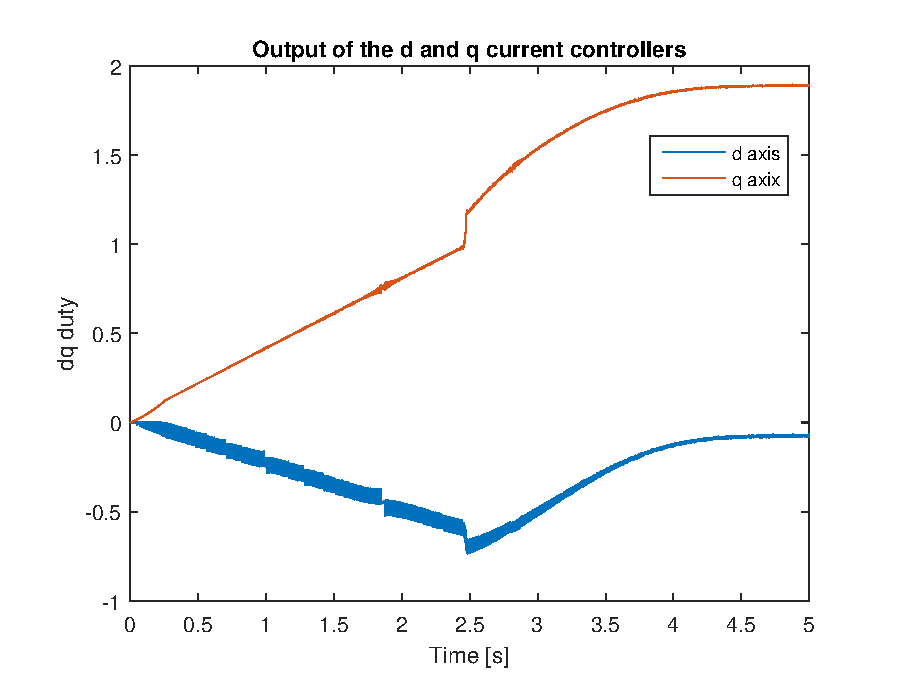
\includegraphics[width=\textwidth]{graphics/before_saturation}
		\caption{Before parallel scale down}
		\label{fig:before_saturation}
	\end{subfigure}
	\begin{subfigure}[t]{.49\linewidth}
		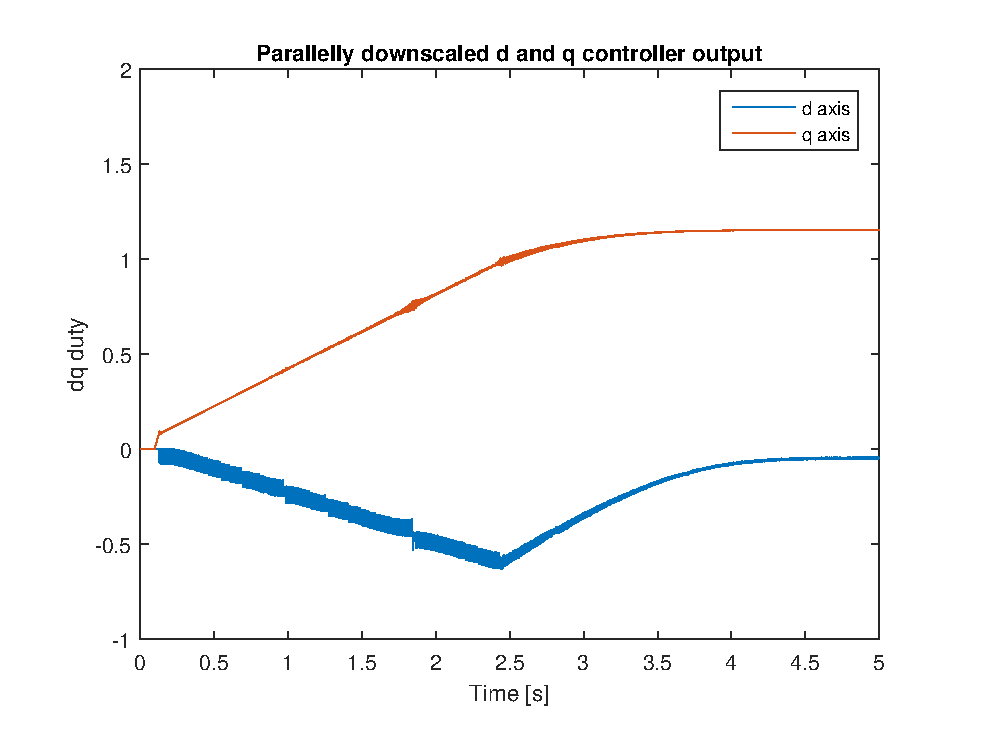
\includegraphics[width=\textwidth]{graphics/after_saturation}
		\caption{After parallel scale down}
		\label{fig:after_saturation}
	\end{subfigure}
	\caption{dq duty cycle values before and after parallel scale down}
	\label{fig:parallel_scale_down_graphs}
\end{figure}

The graphs are simulated with a car mass of 200 kg, and settling time of 0.01 s.
At 2.5 s, the magnitude exceeds $\mathrm{\pm \tfrac{2}{\sqrt{(3)}}}$, at which point both the d and q output is scaled down. 
On figure~\ref{fig:after_saturation}, this transition is almost invisible along the q-curve. 
As the torque produced by the motor is reduced due to saturation of the supply, the need for a large negative d-duty is reduced, as both d and q current is reduced.
This will be explained further on.

Inverse Clark-Park transformation is done by equation~\ref{eq:sim_inverse_clark-park}.

\begin{equation}
\left[ \begin{array}{c}
I_A \\ I_B \\I_C
\end{array} \right]
=
\begin{bmatrix}
\cos (\Phi) & -\sin (\Phi) \\
\cos(\Phi - \gamma) & -\sin(\Phi - \gamma) \\
\cos(\Phi + \gamma) & -\sin( \Phi + \gamma) 
\end{bmatrix}
\cdot
\begin{bmatrix}
I_d \\
I_q
\end{bmatrix}
\label{eq:sim_inverse_clark-park}
\end{equation}

The trigonometric functions used in equation~\ref{eq:sim_inverse_clark-park} are the same as in equation~\ref{eq:sim_clark-park}, so if using lookup-tables, the tables could be reused here. 

\begin{figure}[H]
	\centering
	\includegraphics[width = 14cm]{graphics/sim_PWM_generation}
	\caption{Block diagram of the PWM generator}
	\label{fig:sim_PWM_generation}
\end{figure}

The majority of this block diagram calculates the inverse Clarke-Park transformation, and in the upper right corner, the third harmonic injection is calculated using the knowledge given in the paper 'A Novel Third Harmonic Injection Method for Closed Loop Control of PMSM Motors' \cite{third_harmonic_injection}. \\

The issue is that, when using field oriented control, the stator voltage does not remain at a constant angle relative to the rotor angle.
That means, that calculating the third harmonic isn't as simple as multiplying the rotor position with three. 
Doing this will result in the the third harmonic being out of phase with the three sinusoidal voltage waveforms as speed increases.
This will result in higher peak voltages at certain speeds.
Instead, the third harmonic needs to be calculated from the dq output from the controller. \\

Equation (9) in the paper\cite{third_harmonic_injection} defines the three phase voltage of a balances system without third harmonic injection:

\begin{equation}
\left[ \begin{array}{c}
V_A \\ V_B \\V_C
\end{array} \right]
=
\left[ \begin{array}{c}
V \sin(\Theta) \\
V \sin(\Theta - 120 \si{\degree}) \\
V \sin(\Theta + 120 \si{\degree})
\end{array} \right]
\label{eq:equation_9}
\end{equation}

where $\mathrm{\Theta}$ is the instantaneous phase, and V is the instantaneous magnitude, calculated as:

\begin{equation}
V = \sqrt{V_q ^2 + V_d ^2}
\label{eq:v_from_vdq}
\end{equation}

Note that equation~\ref{eq:v_from_vdq} is not equal to equation 10 in the paper\cite{third_harmonic_injection}, because this dividing with 1.5 is done in the Clarke-Park transform block. 

From equation~\ref{eq:equation_9}, we know that:

\begin{equation}
\Theta = \sin^{-1} \Big(\frac{V_A}{V}\Big)
\label{eq:equation_11}
\end{equation}

The third harmonic sinusoidal is given in equation (12) of the paper\cite{third_harmonic_injection}, and shown in equation~\ref{eq:v_th}

\begin{equation}
V_{th} = \frac{1}{6} \sin(3 \Theta) = \frac{1}{6} \sin\Bigg(3 \sin^{-1} \Big(\frac{V_A}{V}\Big)\Bigg)
\label{eq:v_th} 
\end{equation}

This third harmonic sinus is added to each of the phases, as shown in equation~\ref{eq:equations_14}

\begin{equation}
\begin{bmatrix}
V_{Ath} \\
V_{Bth} \\
V_{Cth}
\end{bmatrix}
=
\begin{bmatrix}
V_A + V_{th} \\
V_B + V_{th} \\
V_C + V_{th}
\end{bmatrix}
\label{eq:equations_14}
\end{equation}

This allows the controller to go beyond the full range of the voltage without saturating. \\

The reason this third harmonic injection is only enabled when the magnitude is larger than zero is to avoid dividing by a negative number in equation~\ref{eq:equation_11}.

\subsection{Simulink Simulation Results}\label{sub:simulink_results}

As stated earlier, the simulink simulation is used to test how the controller handles the five events stated on page~\pageref{sec:Simulations}.
The simulation will be run with both PI and IP controllers, with values described in sections~\ref{sub:full_order_controller_values} and~\ref{sub:reduced_order_controller_values}. \\

At first, a simulation will be run where the throttle is pressed fully from 0.12 s to 5 s, and then released.
The load is 200 kg, which is enough to guard against wheel spin.
The resultant current along the d and q axes have been plotted in figure~\ref{fig:Sim_results_pi_Idq}.

\begin{figure}[H]
	\centering
	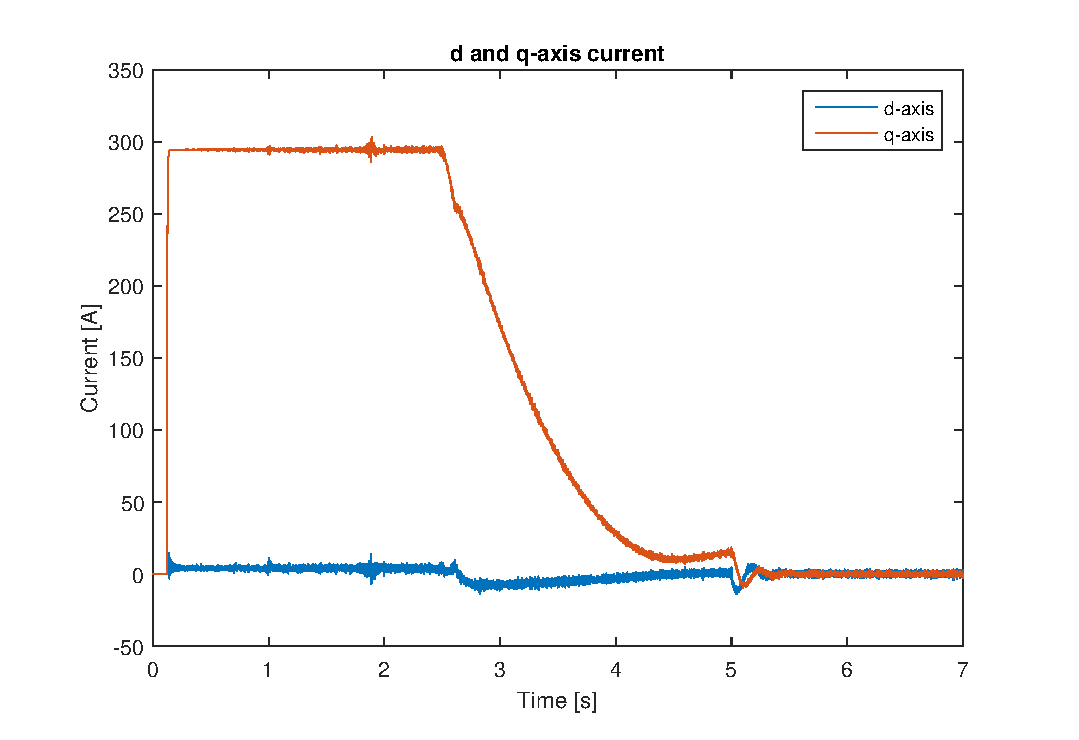
\includegraphics[width=0.7\linewidth]{graphics/Sim_results_pi_Idq}
	\caption{d and q current simulated with a positive and negative step}
	\label{fig:Sim_results_pi_Idq}
\end{figure}

Much like on figure~\ref{fig:Output_Full}, the current steps up nicely with almost no overshoot. 
There is also a small steady state error of about 2 \%.
meanwhile, the d-axis current is kept very low, at least until 2.6 seconds, when the voltage starts saturating. 
A small undershoot is not a big issue, as this is likely to occur if the position encoder is not perfectly aligned.
When saturation occurs, the current drops off almost exponentially. 
As the speed increases, the voltage needed to produce torque lowers until it's only enough to compensate for the drag.
At 5 seconds, when the throttle is released, both the d and q current ripples a bit. 
This is due to the way saturation is handled, but it's not a major ground for concern.

The voltage waveforms must not be saturated, and should remain sinusoidal with third harmonic injection.
This is shown on figure~\ref{fig:Sim_results_pi_phase_voltage}

\begin{figure}[H]
	\centering
	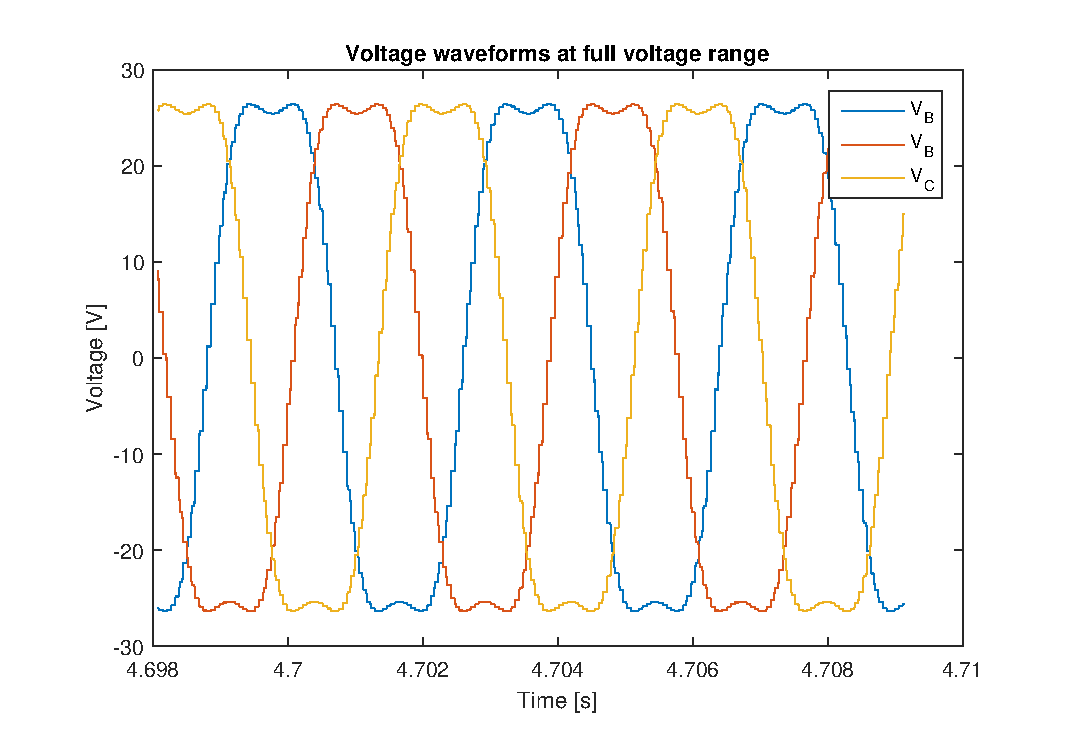
\includegraphics[width = 0.7\linewidth]{graphics/Sim_results_pi_phase_voltage}
	\caption{Voltage waveforms measured when the motor is running at 4000 RPM}
	\label{fig:Sim_results_pi_phase_voltage}
\end{figure}

The reason for is the limited resolution of the encoder. 

When the throttle is released after 5 s, the power should ideally not become negative.




\subsection{Plecs model}\label{sub:sim_plecs_electrical}
As previously mentioned, the Plecs model differs vastly from the Simulink model in the electrical network, as it more closely resembles the real analog circuit. 
It is shown on figure~\ref{fig:plecs_electrical}.
\todo[inline]{Thomas: This needs something more.. Martin: ya think? Thomas: I think...}
\begin{figure}[H]
	\begin{center}
		\includegraphics[width = \textwidth]{graphics/Plecs_electrical.pdf}
		\caption{Block diagram for the svm plecs simlations.}
		\label{fig:plecs_electrical}
	\end{center}
\end{figure}

\subsection{Simulation of the Over-Current Protection Circuit}
\todo[inline]{Thomas: I'm not sure the placement of this makes sense..}
In order to verify the functionality of the OCP circuit discussed in section \ref{sec:ocpcircuit}, simulations of the circuit were conducted in LTSpice\footnote{LTSpice: Free simulation software by Linear Technologies.}.
The results of the simulation will be discussed in the order of the circuit.
As mentioned, only two of the phases are measured and the third will have to be calculated. 
This is done using the summing amplifier circuit shown in section \ref{sec:ocpcircuit}, repeated in figure \ref{fig:sumsimamp} for convenience.
The resulting signals can be seen on figure \ref{fig:sumsimresults}.
Clearly, P3 is not phase shifted 120\si{\degree} with respect to P1 or P2.
This is a consequence of using the non-inverting summing amplifier.

\begin{figure}[!h]
	\begin{subfigure}[b]{0.4\linewidth}
		\centering
		\includegraphics[width=\linewidth,trim=10cm 7.5cm 10cm 8cm]{graphics/sumamp}
		\caption{}
		\label{fig:sumsimamp}
	\end{subfigure}
	\begin{subfigure}[b]{0.6\linewidth}
		\centering
		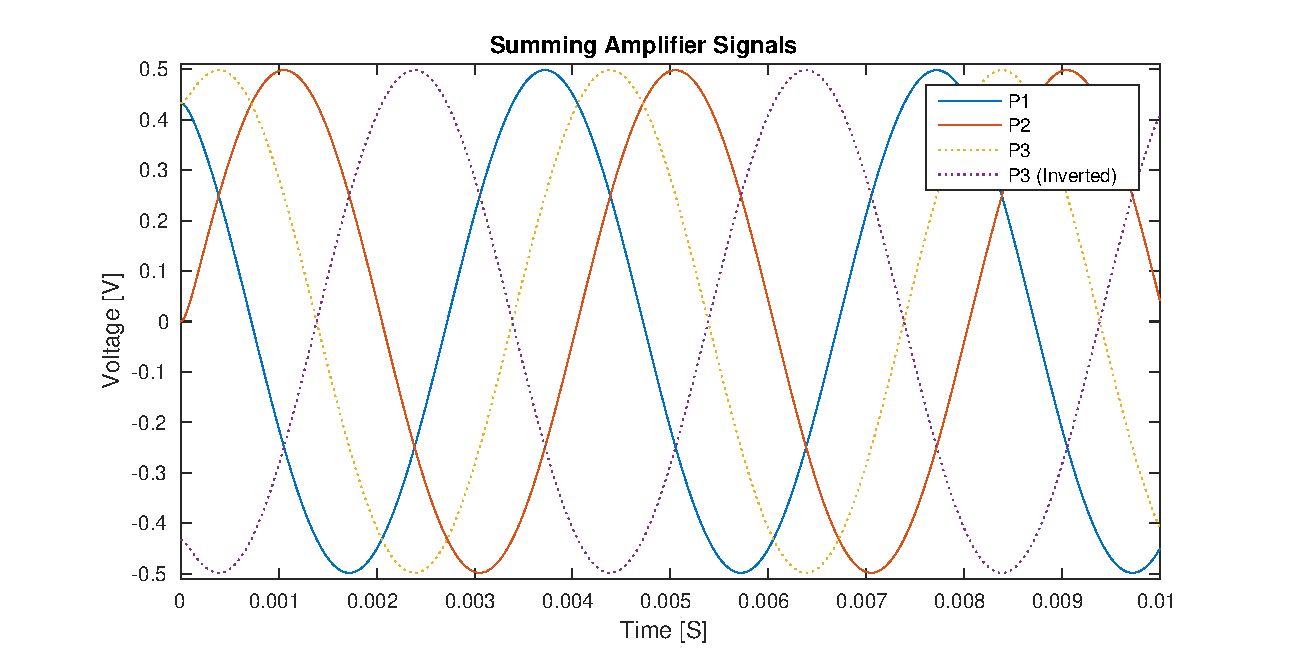
\includegraphics[width=\linewidth]{graphics/sumulation}
		\caption{}	
		\label{fig:sumsimresults}
	\end{subfigure}
	\caption{In \ref{fig:sumsimamp} is shown the summing amplifier used. In \ref{fig:sumsimresults} P1 and P2 represent the two measured phases while P3 is the calculated, third phase.}
	\label{fig:sumsim}
\end{figure}

Inverting P3 however, reveals the correct signal.
As all three signals, P1, P2 and P3 are rectified in the next step, this discrepancy is irrelevant.
For the remainder of this section only one phase is discussed as the circuitry of all three phases is identical after the initial summation.\\

The next step in the OCP process is the rectification of the signals.
This is done using a precision full wave rectifier as shown in figure \ref{fig:fullwaverectifier}.
As can be seen, the rectification error is relatively minor compared to the signal size.
It is mostly caused by the phase shifting done by the rectifier circuit.
This is apparent when noticing that the error is mostly identical between the rectified and non-rectified parts of the signal.

\begin{figure}[!h]
	\begin{subfigure}[b]{\linewidth}
		\centering
		\includegraphics[width=.75\linewidth, trim=0cm 2cm 0cm 2cm]{graphics/fullwaverectifier}
		\caption{}
		\label{fig:fullwaverectifier}
	\end{subfigure}
	\begin{subfigure}[b]{\linewidth}
		\centering
		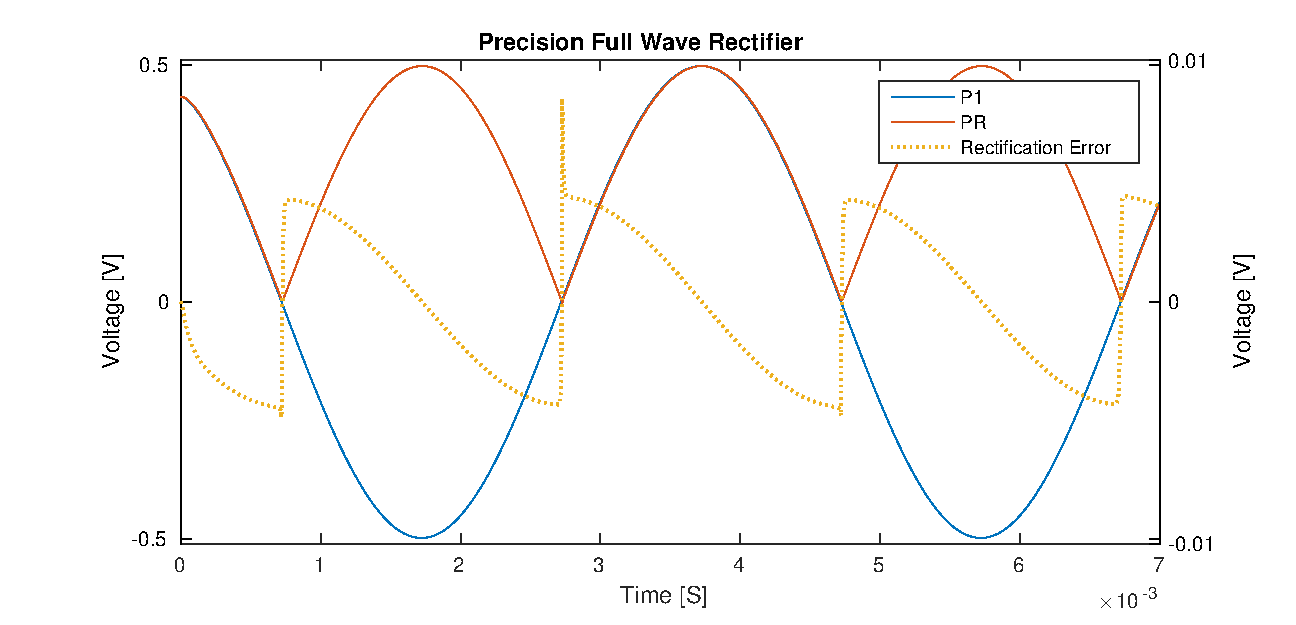
\includegraphics[width=\linewidth]{graphics/fullwaverectifiersim}
		\caption{}	
		\label{fig:fullwaverectifiersim}
	\end{subfigure}
	\caption{\ref{fig:fullwaverectifier} is the the full wave rectifier used to rectify the current signals. \ref{fig:fullwaverectifiersim} shows the rectified version, PR, of one of the phase signals, P1, as well as the error of the rectification.}
	\label{fig:rectifiersim}
\end{figure}

\todo[inline]{Thomas: It would be nice to have numbers on the simulated phase shift done by the recifier.}

After rectification, the signal is fed to a Schmitt-trigger with hysteresis voltages $V_h=0.475\si{\volt}$ and $V_l=0.25\si{\volt}$.
These signals are shown in figure \ref{fig:schmitt}.

\begin{figure}
	\centering
	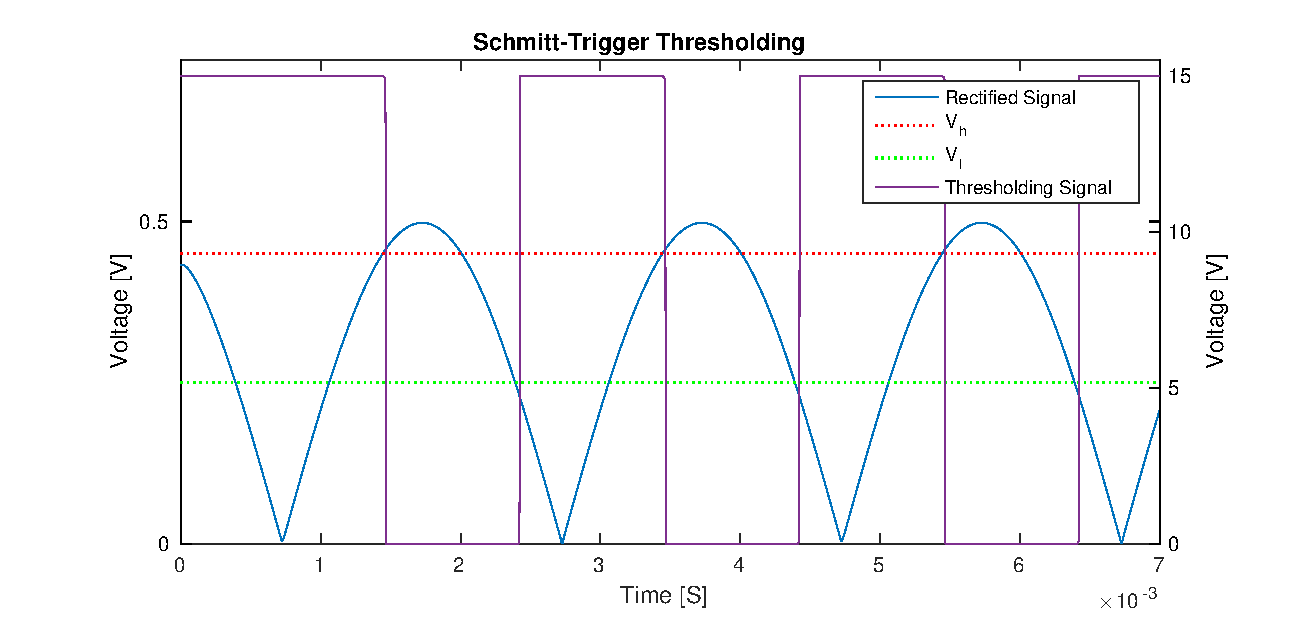
\includegraphics[width=\linewidth]{graphics/schmitt}
	\caption{Thresholding of the phase signals.}
	\label{fig:schmitt}
\end{figure} 